\section{Diskussion}

\subsection{Kvalitet af sCT}


Vi har genereret en del flere sCT som ikke er blevet brugt i rekonstruktioner,  og de fleste er blevet af ret god kvalitet, som kan ses på figur~\ref{col:loocv_ct}. Omkring 20\% af sCT billederne har dog større problemer i selve hjernen.

\begin{figure}
   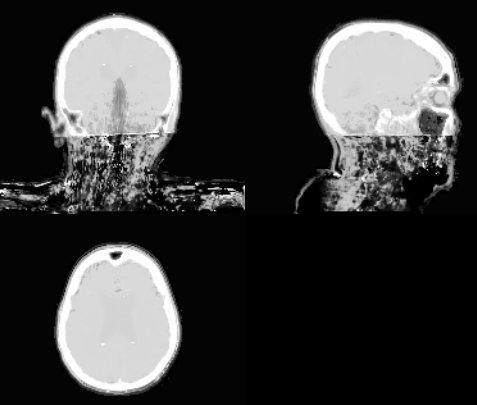
\includegraphics[width=\textwidth]{billeder/sct_problemer.png}
   \caption{sCT med problemer i hjernen. Der er mange punkter med både meget lave og meget høje værdier spredt rundt i selve hjernen.}
   \label{sct_problemer}
\end{figure}

På figur~\ref{sct_problemer} kan man se mange steder med lave værdier mellem knoglen og hjernen. Også inde i midten af hjernen er der problemer med både for høje og lave værdier. Vi er ikke klar over hvorfor nogen patienter bliver meget dårligere end de fleste andre, men Johansson et al. nævner at der kan være problemer med sampling mønstret for UTE sekvenserne.

På en del af billederne er det muligt at se ventriklerne, hvilket man ikke kan på CT billederne i samme grad.

Et væsentligt problem for sCT billederne ligger i at knoglerne bliver tykkere end på de rigtige CT billeder. Det kan ses på differens billederne på figure~\ref{col:loocv_ct_pat1_sub},~\ref{col:loocv_ct_pat1_sub},~\ref{col:loocv_ct_pat2_sub},~\ref{col:loocv_ct_pat3_sub},~\ref{col:loocv_ct_pat4_sub},~\ref{col:loocv_ct_pat5_sub}, da der en to lyse streger rundt om kraniet. Til gengæld ligger værdierne for sCT knoglerne i gennemsnit under værdierne i CT knoglerne, hvilket kan ses på farverne imellem figurene~\ref{col:loocv_ct_pat1_ct},~\ref{col:loocv_ct_pat2_ct},~\ref{col:loocv_ct_pat3_ct},~\ref{col:loocv_ct_pat4_ct},~\ref{col:loocv_ct_pat5_ct} og figurene~\ref{col:loocv_ct_pat1_sct},~\ref{col:loocv_ct_pat2_sct},~\ref{col:loocv_ct_pat3_sct},~\ref{col:loocv_ct_pat4_sct},~\ref{col:loocv_ct_pat5_sct}. Derfor ved vi ikke om det har en stor eller lille indflydelse på PET rekonstruktionen.

\begin{figure}
    \centering
    \begin{subfigure}[b]{0.3\textwidth}
        \centering
        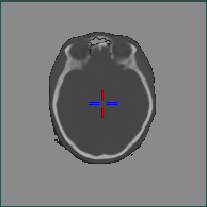
\includegraphics[width=0.75\textwidth]{colager/loocv_ct/loocv_010476_ct.png}
        \caption{CT for patient 1.}
        \label{col:loocv_ct_pat1_ct}
    \end{subfigure}\hfill
    \begin{subfigure}[b]{0.3\textwidth}
        \centering
        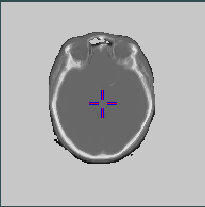
\includegraphics[width=0.75\textwidth]{colager/loocv_ct/loocv_010476_sct.png}
        \caption{sCT.}
        \label{col:loocv_ct_pat1_sct}
    \end{subfigure}\hfill
    \begin{subfigure}[b]{0.3\textwidth}
        \centering
        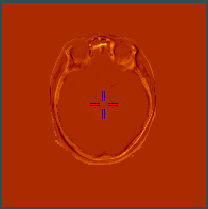
\includegraphics[width=0.75\textwidth]{colager/loocv_ct/loocv_010476_sub.png}
        \caption{Differens.}
        \label{col:loocv_ct_pat1_sub}
    \end{subfigure}\\
    \begin{subfigure}[b]{0.3\textwidth}
        \centering
        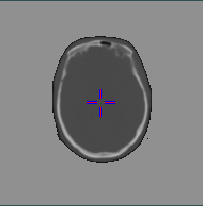
\includegraphics[width=0.75\textwidth]{colager/loocv_ct/loocv_010769_ct.png}
        \caption{CT for patient 2.}
        \label{col:loocv_ct_pat2_ct}
    \end{subfigure}\hfill
    \begin{subfigure}[b]{0.3\textwidth}
        \centering
        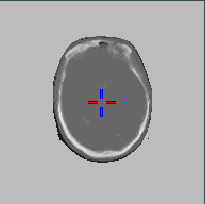
\includegraphics[width=0.75\textwidth]{colager/loocv_ct/loocv_010769_sct.png}
        \caption{sCT.}
        \label{col:loocv_ct_pat2_sct}
    \end{subfigure}\hfill
    \begin{subfigure}[b]{0.3\textwidth}
        \centering
        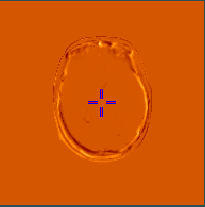
\includegraphics[width=0.75\textwidth]{colager/loocv_ct/loocv_010769_sub.png}
        \caption{Differens.}
        \label{col:loocv_ct_pat2_sub}
    \end{subfigure}\\
    \begin{subfigure}[b]{0.3\textwidth}
        \centering
        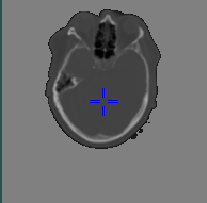
\includegraphics[width=0.75\textwidth]{colager/loocv_ct/loocv_010850_ct.png}
        \caption{CT for patient 3.}
        \label{col:loocv_ct_pat3_ct}
    \end{subfigure}\hfill
    \begin{subfigure}[b]{0.3\textwidth}
        \centering
        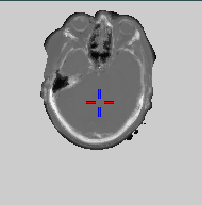
\includegraphics[width=0.75\textwidth]{colager/loocv_ct/loocv_010850_sct.png}
        \caption{sCT.}
        \label{col:loocv_ct_pat3_sct}
    \end{subfigure}\hfill
    \begin{subfigure}[b]{0.3\textwidth}
        \centering
        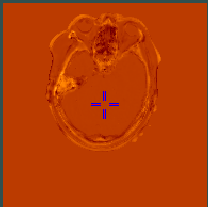
\includegraphics[width=0.75\textwidth]{colager/loocv_ct/loocv_010850_sub.png}
        \caption{Differens.}
        \label{col:loocv_ct_pat3_sub}
    \end{subfigure}\\
    \begin{subfigure}[b]{0.3\textwidth}
        \centering
        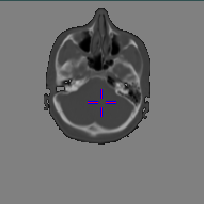
\includegraphics[width=0.75\textwidth]{colager/loocv_ct/loocv_010960_ct.png}
        \caption{CT for patient 4.}
        \label{col:loocv_ct_pat4_ct}
    \end{subfigure}\hfill
    \begin{subfigure}[b]{0.3\textwidth}
        \centering
        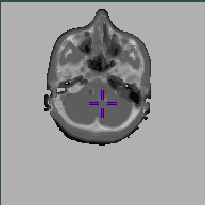
\includegraphics[width=0.75\textwidth]{colager/loocv_ct/loocv_010960_sct.png}
        \caption{sCT.}
        \label{col:loocv_ct_pat4_sct}
    \end{subfigure}\hfill
    \begin{subfigure}[b]{0.3\textwidth}
        \centering
        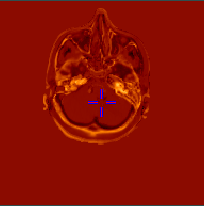
\includegraphics[width=0.75\textwidth]{colager/loocv_ct/loocv_010960_sub.png}
        \caption{Differens.}
        \label{col:loocv_ct_pat4_sub}
    \end{subfigure}\\
    \begin{subfigure}[b]{0.3\textwidth}
        \centering
        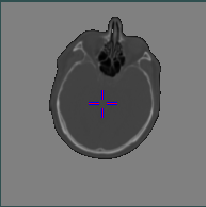
\includegraphics[width=0.75\textwidth]{colager/loocv_ct/loocv_011030_ct.png}
        \caption{CT for patient 5.}
        \label{col:loocv_ct_pat5_ct}
    \end{subfigure}\hfill
    \begin{subfigure}[b]{0.3\textwidth}
        \centering
        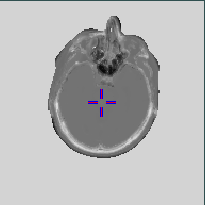
\includegraphics[width=0.75\textwidth]{colager/loocv_ct/loocv_011030_sct.png}
        \caption{sCT.}
        \label{col:loocv_ct_pat5_sct}
    \end{subfigure}\hfill
    \begin{subfigure}[b]{0.3\textwidth}
        \centering
        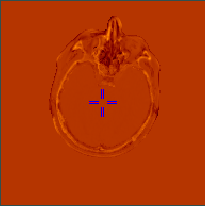
\includegraphics[width=0.75\textwidth]{colager/loocv_ct/loocv_011030_sub.png}
        \caption{Differens.}
        \label{col:loocv_ct_pat5_sub}
    \end{subfigure}
    \caption{CT, sCT og differencen imellem dem for de fem patienter.}
    \label{col:loocv_ct}
\end{figure}

\subsection{Sammenligning med Johansson et al}


Som det ses på figur~\ref{fig:cumm_diff_loocv} er de fleste af vores sCT dårligere kvalitet i forhold til Johansson et al. Patient 1 følger nogenlunde samme kurve som Johansson et al. har fundet frem til. Ligeledes, hvis vi ser på figur~\ref{fig:loocv_j_h}, får vi samme features som Johansson et al. fremhæver.


Vi er ikke sikre på hvorfor vores de fleste af vores sCT er blevet dårligere. Vi tror det er en kombination af flere ting. 


For det første er vores masker ikke optimale, hvilket kan resultere i dårlige modeller. For det andet kan registreringen af sCT og CT ligge en smule forkert. Eftersom vi sammenligner på voxel niveau kræver det at registreringen er så tæt på perfekt som muligt, hvis alt er forskudt bare en enkelt voxel kan det gøre en stor forskel. For det tredje har de formentligt brugt patienter med bedre T2 billeder.


Dog mener vi ikke det har noget med algoritmen at gøre. Vi bruger EM, initialiseret med k-means, hvilket gerne skulle give det samme output hver gang. Da Johansson et al. bruger samme fremgangsmetode mener vi derfor problemet ligger i forbehandlingen af billederne.


Vi prøvede at træne med dobbelt så mange patienter, for at se om det gav bedre resultater, men det havde ikke nogen mærkbar effekt på sCT billederne.


\subsection{Billedformater}

I løbet af projektet har vi oplevet en del problemer med konverteringer
mellem filtyper. Vi benyttertre forskellige. Siemens scannerne producerer
Dicom billeder som vi arbejder med i Osirix, der er et medicinsk
billedbehandlisk program. Men det er et meget stort format, der ikke er
let at arbejde med. 

På Rigshospitalet er normen at konvertere til Minc, men vi havde planer,
om at bruge ITK, og Nifti var bedre understøttet i det. I sidste ende
endte vi med at registrere vores CT billeder i Minc, så vores billeder gik
igennem alle tre typer. 

Fra Dicom til Minc mister man en skalar, som man skal tage højde for, når
man konvertere tilbage. Ved konvertering fra Minc til Nifti, hvilket vi
kun gør med vores registrerede CT billeder, bliver de laveste værdier til
-1024, dem trækker vi endnu 1025 fra, så de kommer til at matche vores
laveste værdier.

\todo{Uddyb tab ved Dicom til Minc}

At konvertere til Dicom er ikke helt trivielt, så vi konverterer først til
Minc, hvor vi lægger 2048 til for at gøre op for det offset, der skete ved
den tidligere konvertering. 

Mange af disse problemer har vi opdaget så sent i processen, at vi ikke
har kunnet nå at tage hånd om dem. Den gennemsnitlige værdi i alle vores
Nifti billeder, som vi har trænet og testet på, har været for lav, og at
lægge en værdi til ved tilbagekonverteringen udbedrer det ikke, men ændrer
bare værdierne til samme størrelse, som i det målte CT.


\subsection{Fullct-PET og sCT-PET kvalitet}


Værdierne i et PET-billede kan ikke sammenlignes direkte på tværs af patienter, de har kun betydning i forhold til resten af hjernen. Så hvis det forreste af hjernen, for eksempel, afviger mere fra resten af hjernen end normalt, så er der et problem der. På samme måde er det ikke noget problem, hvis de rekonstruerede PET billeder baseret på sCT afviger med en relativ faktor i hele hjernen i forhold til dem baseret på FullCT. På figur~\ref{col:loocv_pet} ses der på procentdifferensbillederne en nogenlunde jævn grøn nuance i det meste af hjernen (pånær patient 5), hvilket taler for kvaliteten af resultaterne. 


Vi oplever store forskelle i ventriklerne, som set på figur~\ref{col:loocv_pet_pat3_pd}~og~\ref{col:loocv_pet_pat3_pd}  men det er ikke noget problem. De består hovedsageligt af vand, og der foregår ikke nogen aktivitet i dem. Derfor er værdierne i ventriklerne meget lave, så afvigelser vil give større udslag der end andre steder i hjernen. I det hele taget er forskelle i alt andet end selve hjernen ikke relevant. Hvis selve knoglen giver store udslag, eller der er problemer i ansigtet betyder det ikke noget.


I forhold til vores ønske, om at holde forskellen under 5 \% eller i hvert fald 10 \%  er det ikke lykkedes. Bagerst i hjernen ser det meget godt ud, men i regionerne ved øjnene og i lillehjernen ser vi i snit en procentdifference på over 5 \% i mere end en femtedel af voxelsne (~\ref{tab:loocv_lillehjerne} og \ref{tab:loocv_lillehjerne}). På figur~\ref{col:loocv_pet_pat3_pd} og~\ref{col:loocv_pet_pat5_pd}  kan man se en hvide bjælke med forskelle på over 20 \%, der matcher, hvor T2’en slutter. Bjælken går igennem lillehjernen, og resultaterne bliver derfor kraftigt forværet, som set på figur~\ref{tab:loocv_lillehjerne}. Det er også tydeligt at se på figur~\ref{col:loocv_pet_pat3_pd} og~\ref{col:loocv_pet_pat4_pd} at der mangler T2 værdier ved den øverste del af kraniet.


Derudover kan vi på figur~\ref{tab:loocv_forresthjerne} og figur~\ref{tab:loocv_lillehjerne} se at halvdelen af patienterne har store problemer forrest i hjernen og ved lillehjernen. Dette tyder på vi i yder områderne ikke kan hamle op med PET baseret på FullCT’et. Dette kan også ses på billeder ne i figur~\ref{col:loocv_pet_pat1_pd} og figur~\ref{col:loocv_pet_pat3_pd} hvor forskellen er større i den forreste del af hjernen i forhold til resten.

\subsection{Over tid}

På figur~\ref{col:over_time_sct} kan ses de producerede sCT’er ud fra
de to modeller. Det er iøjnefaldende at dem lavet ud fra den sene model
har meget tydeligt markeret fejl ind i hovedet, mens der de samme
steder i dem fra den tidlige model er langt svagere strukturer. Udover
det er de sene også mørkere, og har dermed lavere værdier. Vi må
konstatere at modellerne producerer ret forskelligt artede resultater.
Vi har ikke håndplukket vores hjerner, men blot valgte de tidligste
og seneste uden artefakter til at træne på, så det er muligt, at
den ene model er bedre end den anden. Patient tre mangler desuden
bunden af lillehjernen på T2-sekvensen, så formodentlig vil der være
attenuationsproblemer i bunden af PET billedet.

På figur~\ref{col:over_time_pet_pat1_pd} og
figur~\ref{col:over_time_pet_pat2_pd} kan man se en jævn forskel i hele
hjernen. På patient 2 kan man langs med den øverste kant se en større
forskel. Det samme gør sig i mindre grad også gældende for de andre.
På patient 3 figur~\ref{col:over_time_pet_pat3_pd} er der mærkbare
udslag i billedet. Det bliver specielt et problem ved lillehjernen, hvor
der opstår forskelle på over 20 \%. Dette skyldes, at lillehjernen
er mindre på billedet lavet ud fra modellen trænet på sene hjerner
figur~\ref{col:over_time_pet_pat3_late} end den fra de tidlige
figur~\ref{col:over_time_pet_pat3_early}.

Hvis Patient 3’s store udslag er et enkeltstående tilfælde, eller
blot flot en fejl fremprovokeret af en dårlig model, så er billederne
formodentlig lig nok til, at man ikke behøver at gentræne modeller
løbene. Udslagene i mellem billederne er nogenlunde jævnt fordelt, så
der er ikke problematiske. I kanterne har vi generelt samme problemer
som vi ser i LOOCV-forsøget, så selvom der sker ændringer der, kan vi
ikke påvise, om de bliver bedre eller dårligere.

\subsection{Klinisk anvendelighed}

Så kommer det store spørgsmål - kan sCT bruges klinisk ?  Ifølge Ian Law, overlæge på rigshospitalet, så ser billederne fornuftige ud for nogen patienter men mindre brugbare for andre. PET billeder tages med forskellige typer af sporstoffer der bruges til forskellige diagnosticeringer. Han mener at vores sCT kunne bruges sammen med sporstoffet FDG, hvilket bliver brugt til diagnosticering af alzheimers. FDG er interessant fordi vi ikke leder efter små uregelmæssigheder, som for eksempel en kræftcelle, men er mere interesseret i hele regioners optag i forhold til resten af hjernen. Vi har udelukkende brugt FDG patienter i vores forsøg, men det skyldes at Rigshospitalet har flest FDG patienter. Eftersom det kun tager få minutter at generere et sCT ville det også være muligt at inspicere sCT’et inden man tager et CT billede. Hvis der ingen synlige problemer med sCT billedet er, kunne det bruges til rekonstruktionen. Omvendt, hvis der er problemer kunne man derefter tage CT billedet.

På den anden side, så fortæller vores procentdifferensbilleder en anden historie. Vi har vist at der er store problemer i den forreste del af hjernen, og kvaliteten ser ikke ud til at være stabil. Det er muligt at man kan finde en model, der virker godt på langt de fleste patienter og dermed gøre sCT mere brugbare.

Vi har ikke kigget på patienter med artefakter på MR billederne, men omtrent halvdelen har artefakter. Vi er ret sikre på at artefakter i MR billederne vil resultere i ens artefakter i sCT billederne. Dermed bliver anvendeligheden af sCT reduceret en del, eftersom CT ikke vil have artefakterne.
